\section{FFS}
The artifact that was developed as a result of this thesis is the Fejk FileSystem (FFS). It used online services to store the data but behaved as a mountable filesystem for the users. The filesystem will be minimal and not support all functionalities that other filesystems do, such as links. The reasoning is that these behaviors are not required for a useable system, and when comparing the system to distributed filesystems such as Google Drive, many of these other filesystems also often do not support links.

\subsection{Design overview}
FFS will use images and text to store the data of files, directories and the inode table. These images and texts will can be uploaded to online web services, such as Twitter, as image posts or text posts. As mentioned in Section~\ref{sec:twitter}, there can be limitations to these posts for certain online web services. To support file sizes bigger than these limitations, bigger files will be split into multiple posts, requiring FFS to keep track of a list of posts. Figure~\ref{fig:ffs_inode_diag} presents the basic outline of FFS and a example content of the filesystem. FFS is based on the idea of inode filesystems and uses a inode table to store information about the files and directories in the filesystem. However, instead of an inode pointing to specific blocks in a disk, the inode table of FFS will instead keep track of the id numbers of the posts on the online services where the file or directory is located. The inode table entry for each file or directory will also contain metadata about the entry, such as its size and a boolean indicating if the entry is a directory or not.

\begin{figure}[!ht]
	\begin{center}
	  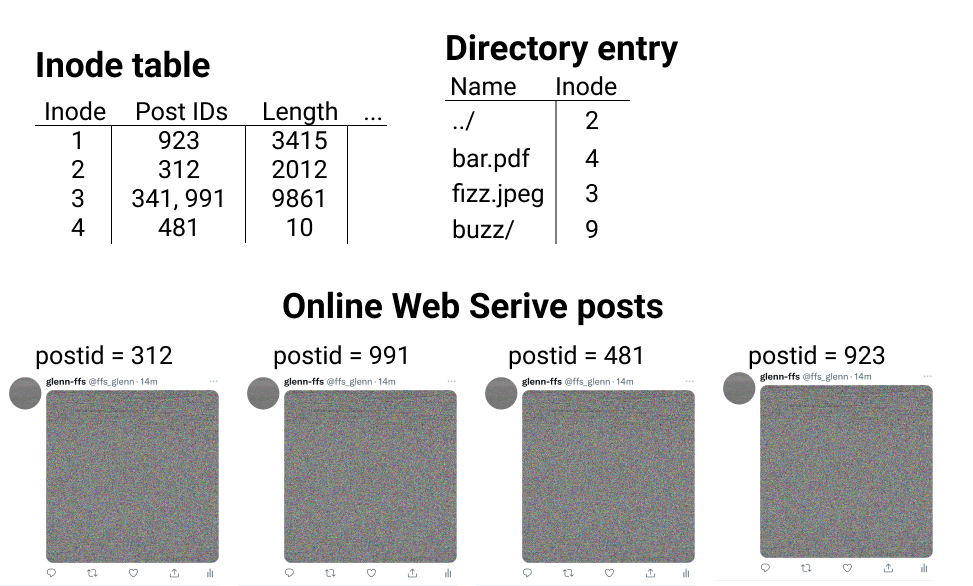
\includegraphics[width=0.8\textwidth]{figures/ffs_inode_diagram.png}
	\end{center}
	\caption{Basic structure of FFS inode-based structure}
	\label{fig:ffs_inode_diag}
\end{figure}

The directories and inode table are represented as classes in C++. Appendix~\ref{lst:dir_itable_classes} visualizes the main attributes of the \texttt{Directory}, \texttt{InodeTable}, and \texttt{InodeEntry} classes. There can be multiple \texttt{Directory} and \texttt{InodeEntry} objects in memory and in the filesystem, but there will only be one \texttt{InodeTable}.

\subsection{Encoding and decoding objects}
Objects that FFS store, and therefore also encode and decode, are: files, directories and the inode table. All of these objects are stored on online web services using images and texts. The inode table and the directories are represented as C++ objects in memory, but are serialized into a binary representation during runtime before encoded into images or text. The files saved in FFS are also read into memory in a binary format before being encoded and uploaded to the online web services.


% As a deniable filesystem, you should not be able to gain any information about the filesystem without the correct credentials. Using incorrect credentials, the filesystem will just show an empty filesystem meaning that the adversary will not know wether the credentials provided were correct and that the filesystem is empty, or if the credentials were incorrect. Only when the correct credentials are provided will FFS show the filesystem contents of the user.

